\documentclass[twocolumn]{article}  
\setlength\topmargin{0pt}
\addtolength\topmargin{-\headheight}
\addtolength\topmargin{-\headsep}
\setlength\oddsidemargin{0pt}
\setlength\textwidth{\paperwidth}
\addtolength\textwidth{-2in}
\setlength\textheight{\paperheight}
\addtolength\textheight{-2in}
\usepackage{layout}


\usepackage{graphicx}
\usepackage{listings}
\usepackage{syntax}
\usepackage{listing}
\usepackage{url}
\usepackage{framed}
\usepackage{authblk}
\usepackage{amsmath}
\usepackage{verbatim}
\usepackage{hhline}
\usepackage[]{algorithm2e}
\usepackage{makecell}
\usepackage[capposition=bottom, footfont=footnotesize]{floatrow}
\captionsetup{singlelinecheck=on}

\begin{document}

\title{Joint Optimization of Link and Node Resources in a Network}


\author[*]{Moses Charikar}
\author[*]{Yonatan Naamad}
\author[*]{Jennifer Rexford}
\author[*]{Kelvin Zou}
\affil[*]{Department of Computer Science, Princeton University}
\affil[*]{\textit {\{moses,ynaamad,jrex, xuanz\}@cs.princeton.edu}}


\date{}

\maketitle
%\begin{abstract}

%\end{abstract}

\section{Introduction}

Networks today have evolved beyond simple packet forwarding. There are many types of flow processing taking place at different appliances (e.g., firewall, proxy, intrusion detection system) in the networks. People have long treated networks as graph models, max flow and shortest path problems \cite{FordFulkerson, Edmonds1972} have been widely applied in network design and operation. Nevertheless, traditional graph models only focus on flow routing and thus not be able to capture the whole story. We should also consider flows' in-network process when designing the graph model. 

Given the prevalence and values of the middleboxes, we argue that they are no longer "second class citizen" in networking design and deployment and should be treated with equal importance when we design a network. In particular, we need to jointly optimize how to route and process the flows during networking design.

Traditionally, those middleboxes had to use specialized hardware to get desirable performance, for instance, transcoding requires high computational power and deep packet inspection consumes a lot of memory. Due to the high cost of the specialized hardware, network designs are restricted by the limited number of middleboxes and their functionalities. Network operators tend to place middlebox with great caution and calculation. In many cases network operators simply place middleboxes at chokepoints such as gateway, so flows can share the use of same middleboxes. Choke point placement achieves efficient usage and coverage of middleboxes, the tradeoff is its vulnerability to single point failure. It also leads to inefficient routing if two hosts are placed at the same side of the choke point. 

Some new approaches use the idea of Software-Defined Network (SDN), and take advantage of its centralized view of network and provide more freedom for middlebox placement while forcefully steering traffic to middleboxes, however this approach inevitably creates excessive bouncing traffic in the network\cite{SIMPLE2013,FLOWTAGS2014}.

One popular trend for networking is virtualization, and people have proposed various designs, e.g., OpenVSwitch\cite{openvswitch}, modular middlebox\cite{COMB2012, clickos}. A middlebox is very suitable for virtualization: unlike the switch or router which only needs simple forwarding actions, middleboxes ask for more advanced functions and are not simply just I/O bounded, CPU and memory in many cases are the bottleneck. As the hardware capability grows and the gap between hardware and software solutions closes, we can expect a broader deployment of virtual middleboxes. 

Though the demand for building network around virtualized middleboxes is growing, people still build the network based on the routers and switches with the same mindset of using physical middlebox, and the solutions for middlebox placement and routing/resource allocation are not very promising. Outsourcing to the cloud or handling at the end machines in an elastic manner has been proposed but it imposes high latency and also results in inefficient routing\cite{APLOMB2012, ANANTA2013}. As virtualization enables elasticity and divisibility, it makes middlebox placement more flexible. Since state-of-the-art server machines can support up to several gigabits per second bandwidth, and some new architectural design can create middlebox VM instances in milliseconds with very low overhead in memory\cite{clickos}, we argue that we can run all middlebox instances anywhere in the network, more specifically we can use server machines to run middleboxes and connect those machines not only to leaf nodes or choke points, but to any network node. By doing this we can: 
\begin{itemize}
\item \textbf{Improve the fault tolerance for in-network process} 

Traditional network meticulously places middlebox at choke points shared by many flow. Our system eliminates the dependency on choke points and therefore immune to single point failure. 
\item \textbf{Reduce unnecessary bouncing traffic} 
 
Current networks steer traffic to middleboxes and may add redundant load on the network and extra latency for each flow. We can take advantage of virtualization and the freedom of middlebox placement to avoid unnecessary traffic bouncing.  
\item \textbf{Ease middlebox policy enforcement and load balancing}

Current middlebox policies are achieved by forcing traffic to go through each middlebox, e.g., if the policy is firewall->proxy, the policy is enforced by steering traffic to firewall first and then proxy. In the new system we can simply run different VM instances at the same node and easily enforce the policy. Dynamic spinning or shutting off a middlebox VM in the network also makes load balancing easier.
\end{itemize} 
We make the following few contributions in this paper, 
\begin{enumerate}
\item We design a graph model and formulate a centralized optimization solution for this model given the new network setup we have.
\item We address some practical problems introduced by the network dynamics, such as traffic size change due to middlebox processing (e.g., compression), policy enforcement for heterogeneous resources.  
\item We design an approximation algorithm to solve offline middlebox placement problem and model the online dynamic change problem.

\end{enumerate}

This paper is structured as the  following: we begins with establishing an optimization model for the network with middleboxes in section 2, In section 3 we propose the solutions for some practical problems encountered in real network. We finalize the design choice for offline middlebox placement problem in section 4. We present future direction for online algorithms in section 5 and conclude in section 6.
 

\section{Network with Link and Node Capacities}
In this section we first bring up the assumptions for our network [section \ref{setup}], and then abstract the problem to a graph model [section \ref{graphmodel}]. We end this section with some analysis of the optimization problem[section \ref{optimization}]. 

\subsection{Network Setup}\label{setup}
Before delving to the graph model, we first clarify the network setup. In the network each link has its bandwidth, and each server machine has its processing capacity. The processing capacity is an abstraction and we can think this as CPU or memory. As we mentioned before, the middleboxes are all virtualized, so middlebox VM instances are sharing the same server machine and thus sharing the same hardware resource capacity. We assume the middlebox processing capacity and demand are homogenous, in addition we can later show heterogenous resource demand and capacity also fits in the setting. 

The network consists of a set of flows, each is represented as $f_i$. A flow in this setting is not a simple TCP flow, but some large traffic aggregate, and therefore all the flows can be treated as infinitely divisible and be split at any place in any fractional manner while ensuring all packets of the same connection traverse the same path. We can think the in-network processing demand as an aggregation of different kinds of middlebox processing demand for $f_i$, and the in-network processing for middlebox is proportional to the flow size, which means a flow of two units require twice as much server machine processing resource as a flow of one unit. This assumption holds for most cases where middleboxes processing is per-packet based. We denote $r_i$ as flow rate for $f_i$, and $d_i$ as in-network processing demand, and we can also derive $q_i = \frac{d_i}{r_i}$ based on the assumption. Our model assumes middleboxes do not change the routing behavior (e.g., Firewall, IDS, IPS, Proxy), but two exceptions NATs and Load Balancers do not apply in our model. 
\begin{figure}
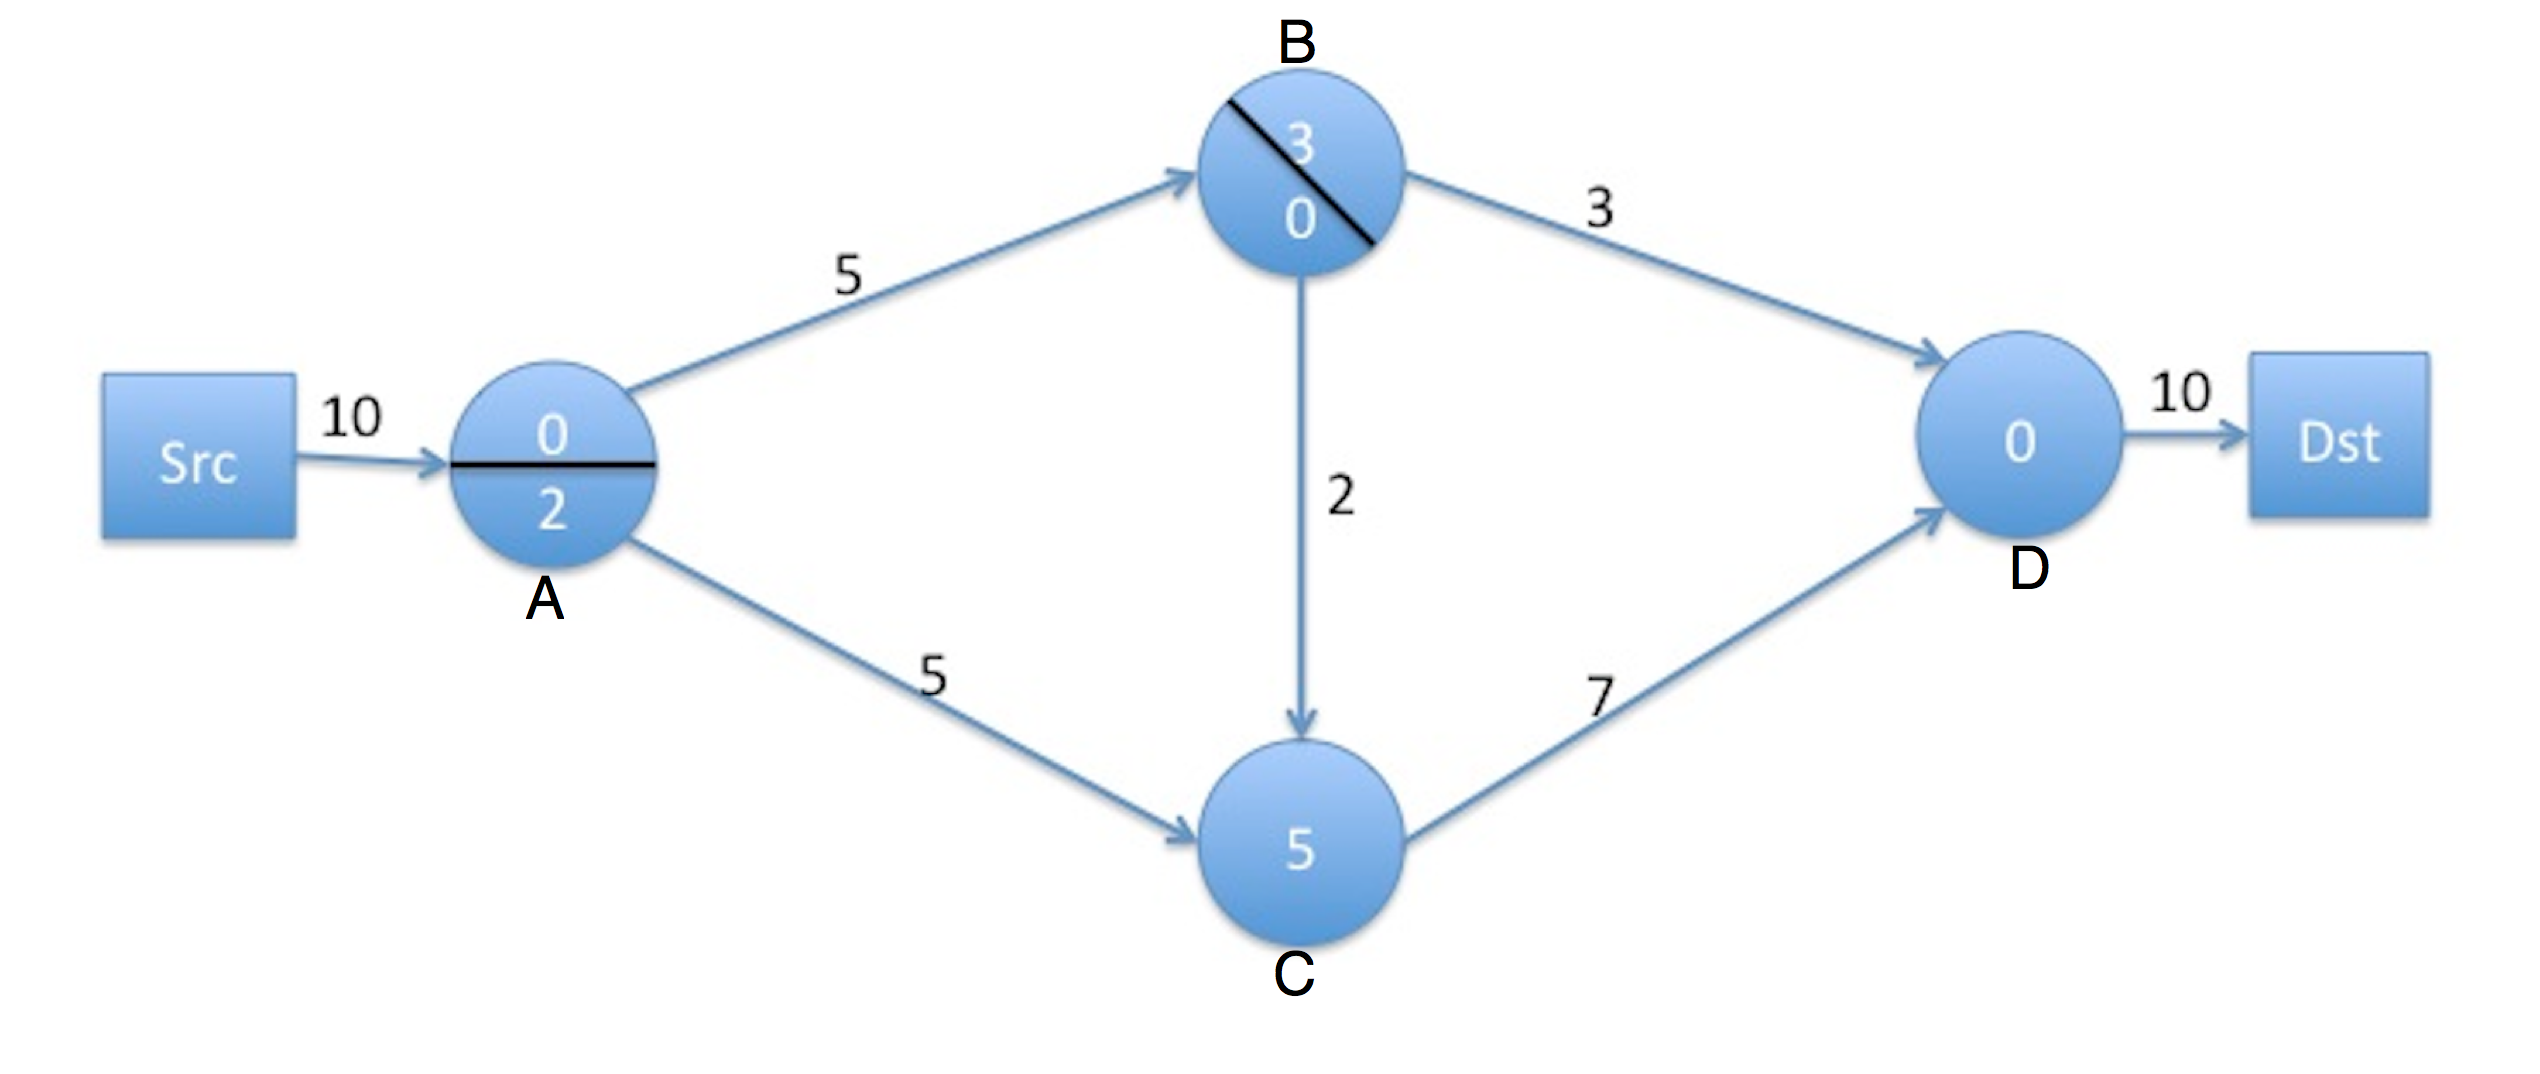
\includegraphics[scale=0.18]{demo.png} 
\caption{ \textbf{Simple example for graph model:} \textit{C(A)=2, C(B) =3, C(C)=5, all B(e) =10, one optimal solution would be 10 units of flow from $src->A$, at A 2 units processed and 3 units unprocessed flows send to C and 5 units unprocessed to B, at B 3 units processed sent to D and 2 units unprocessed to C, at C all units are processed along with 2 already processed flow (from A) sent to D.} \label{demo}}
%\floatfoot{}
 \end{figure}


\subsection{Graph Model}\label{graphmodel}
A traditional network is constrained by link bandwidth: flow feasibility problem is asking whether a flow pattern is feasible given the constraints of link bandwidths. To integrate the middlebox into the graph model, we need to convert middleboxes to node capacity. The node with a capacity can be a server machine in the network or a server machine attached to some node in the network. The role a middlebox plays in a graph is quite different from links so reducing a node with capacity to a virtual link does not work. Unlike the flow without in-network process where the flow is strictly constrained by the bottleneck link bandwidth, in-network processing is handled in a cumulative manner, in other words, for a certain path a flow is constrained by the sum of all processing capacity of node on the path and any link bandwidth on the path. In figure \ref{demo} the graph has link capacity 10 for all links, the processing capacities for node A, B, C, D are 2, 3, 5, 0 respectively. The figure shows 10 units of flow can be sent from the source to the destination and the in-network process is handled in a cumulative way.

In summary we have a graph $G(V,E)$ with both link bandwidth $B(e)$ where $e \in E(u,v)$ and node capacity $C(v)$ where $v \in V$. 
\begin{table*}
\begin{tabular} {|c |c |}
\hline
Notation&Meaning\\ \hline
G(V,E)&Graph G with vertices V and edges E.\\ \hline
B(e)&bandwidth capacity for link $e \in E$\\ \hline
C(v)&middlebox processing capacity at node $v \in V$\\ \hline
$f_i$& Flow i, it is a large traffic aggregate with a certain source and a certain destination\\ \hline
$r_i$&flow sending rate for $f_i$\\ \hline
$d_i$&in-network processing demand for $f_i$\\ \hline
$q_i$&ratio between in-network processing and flow rate\\ \hline
$ f_i(e)$&flow load at edge $e\in E $ for flow i\\ \hline
$ w_i(e)$&in-network process demand at edge e for $f_i$\\ \hline
$p_i(v)$&in-network process handled at node v for $f_i$\\ \hline
$u(e) $&link utilization for edge $ e \in E $\\ \hline
$u(v)$&node utilization for node $ v \in V$\\ \hline
$\phi(u)$&cost function of utilization\\ \hline
$\Phi_e$&cost function for edges, it is the sum over all links' $\phi(u)$\\ \hline
$\Phi_v$&cost function for nodes,  it is the sum over all nodes' $\phi(u)$\\\hline
%\Xhline{3\arrayrulewidth}
\end{tabular}
\centering
\caption{Variables in Graph Model and Optimization Problem}
%\floatfoot{Before the bold horizontal line are notations for pro}
\end{table*}
 
\subsection{Optimization Formulation}\label{optimization}
We first look at the objective function, then establish all constraints based on the graph model in Section 2.1.

The objective we try to achieve in the graph is to minimize the cost for bandwidth consumption and in-network process workload while satisfying the flow and in-network process demands. In the optimization problem we will solve both flow size $f_i(e)$ and un-handled in-network process $w_i(e)$ for each $f_i$ and each edge e. we introduce the two utilizations: 

$u(e) = \frac{\sum\limits_{i} f_{i}(e) } {B(e)}$ and $u(v) = \frac{\sum\limits_{i} p_i(v) } {C(v)} $.

In addition, we introduce a function $\phi(u)$ where it is a concave function for utilization $u$ and $\phi(u)$ goes much steeper as $u$ increases to penalize high utilization. 

The objective function for optimization problem would be to minimize $\Phi_v + \Phi_e$ where $\Phi_e = \sum\limits_{e\in E} \phi_e(u (e) )$ and $\Phi_v = \sum\limits_{v\in V} \phi_v(u (v) )$.

Now let us look at the constraint part. We note that in the formulation simply having values $f_i(e) ,\; p_i(v)$ for each flow $f_i$, edge $e$ and node $v$ fails to provide enough information for routing. The optimization problem needs to tell us exactly which part of in-network process demand from which incoming edge is handled at each node to make the routing and resource allocation decision. We introduce $w_i(e)$ to represent the number of in-network workload demand carried by each edge e, the relation between $p_i(v)$ and $w_i(e)$ is that $p_i(v) =  \sum\limits_{in } w_i(e) -  \sum\limits_{out} w_i(e)$. In addition, the in-network workload demand should be carried by flow, so we need to add extra constraint for each $f_i$: $\forall e; 0\leq w_i(e) \leq q_i*f_i(e)$. Since all the constraints are linear, we can formulate the optimization problem as a linear program:

Minimize  $\Phi_e + \Phi_v$

Subject to:
\begin{subequations}
\begin{align}
&\forall v \in V-\{s, t\}, \forall i, \sum\limits_{in}  f_i(e)=  \sum\limits_{out} f_i(e);\\
&\forall e,\forall  i, f_i(e) \geq 0;\\
&\forall e, u(e) = \frac{\sum\limits_{i} f_{i}(e) } {B(e)};\\
&\forall e,\forall  i, w_i(e) \geq 0,\\
&\forall e,\forall  i, w_i(e) \leq q_i* f_i(e),\\
&\forall v,\forall  i, p_i(v) =  \sum\limits_{in } w_i(e) -  \sum\limits_{out} w_i(e) ;\\
&\forall v,\forall  i, p_i(v) \geq 0; \\
&\forall v, u(v) = \frac{\sum\limits_{i} p_i(v) } {C(v)} ; \\
&\forall i, \sum\limits_v f_i(s, v) = r_i; \\
&\forall e\in(s, v),\forall  i, w_i(e) =q_i* f_i(e);\\
&\forall e\in(v,t), \forall i, w_i(e) =0.
\end{align}
\end{subequations}

The optimization problem gives an output of $p_i(v)$, $f_i(e)$ and $w_i(e)$ and we have formally proved the adequacy of the output for routing and in-network process allocation by showing a way to peel off from this edge based solution to a path based solution. 


\emph{Linear Programming Complexity Analysis}: this optimization formulation is quite similar to traditional traffic engineering problem, where constraints are only 1a, 1b, 1c, 1i. In traditional TE the variable size$=2*E*i=O(E*i)$, and our linear program model contains $5*E*i=O(E*i)$ variables where E is the number of edges and i is the number of flows, so they are at the same complexity level and the input size is 2.5 times the traditional TE matrix. Simplex approach has average case $O(d^2*L)$ where d is the number of variables and L is input bits(in a modern computer it is 32 or 64), so our approach will expect 6.25 times runtime of the traditional TE formulation. If we use strong polynomial solution-interior point approach, then complexity is $O(d^{3.5}*L)$ \cite{InteriorPoint} so our approach will be 25 times more expensive in runtime. Both are reasonable for an offline pre-computation.

\section{Support for Diverse Network Scenarios}
Section 2 tries to capture the core part of a new network model as a flow problem. On top of the core formulation in section \ref{optimization} we show that we can capture a few networking characteristics via some variants of the core formulation. This section starts with the case where flow size might change due to in-network processing[section \ref{size change}]. We also show that the formulation can also capture heterogeneous middlebox processing capacity in a general case[section \ref{Hetero}].


\subsection{Flow Size Change after Processing}\label{size change}
The core model makes the assumption that in-network processing does not affect the traffic size. Nevertheless many types of in-network process change the traffic size, for example, encryption increase the flow size via changing either the header or both header and payload\cite{SIMPLE2013}; compression and transcoding decrease the traffic size by up to a factor of two\cite{Mogul1997}. We need to also capture this in the optimization formulation.

We borrow the idea from LP formulation in generalized circulation cost minimization problem.\cite{Wayne1999} Flow circulation problem computes the minimum cost from a source to a destination given a network wherein there is an upper bound and lower bound for flow size on each link and after each node the flow size is changed by some factor.  One thing different in our model is that flow size change only applies to flows which has not been through in-network process yet. 

We divide the flow into two categories; pre in-network processed, and post in-network processed. They are represented in $f^1$ and $f^2$ respectively. If we put them back to the $f_i, w_i$ presentation, $f_i^1*q=w_i$ and $f_i^2*q_i= f_i *q_i-w_i$ in the initial formulation. If there is a size change, let us introduce a factor $t$ where t represents the ratio between the post in-network and pre in-network processed. $t$ is based on each $f_i$ so each flow has its $t_i$.

If we go back to the core formulation, we need to modify 1a flow conservation constraints, because flow size changes at each hop, incoming flow size is not equal to outgoing flow size anymore. But we can know at each node how much flow exactly changed due to flow size change based on how much in-network process is done from $p_i(v)$ and therefore we can know the "skewed" flow conservation. We can get $\sum\limits_{in} f_i^1(e) - \sum\limits_{out}  f^1_i(e) =\frac{ p_i(v)}{q_i}$ and $\sum\limits_{out} f_i^2(e)-\sum\limits_{in}  f_i^2(e) = \frac{p_i(v)}{q_i}*t_i;\;t>0$. 

We can rewrite 1a to  $\sum\limits_{in} f_i^1(e) - \sum\limits_{out}  f^1_i(e) =(\sum\limits_{out} f_i^2(e)-\sum\limits_{in}  f_i^2(e) )*t_i$. It indeed does not change the complexity of the linear program model.


\subsection{Enforce Policy among Different Middleboxes}\label{Hetero}
In a network, a flow sometimes needs to go through several different in-network processes, e.g., $firewall-IDS-Proxy$. So far we assume the nodes are all homogeneous, which means they can fulfill all types of tasks or processing. However we show that this formulation can generalize the problem, including heterogenous hardware middleboxes can also be captured. If we have specialized hardware for different middleboxes, we will have a new model which contains $C_k(v)$ whereas k represents a type of middlebox processing. 

The in-network processing policy can be captured as a serial processing. If we can have several different types of workloads, $w^a$, $w^b\dots$, to ensure serial processing, aside from the workload constraints enforced at section2.1, we also need additional constraints w.r.t. the order. To make example simple, assume we only have two different types of in-network process, and we want flow go through process $a$ before process $b$, we can simply have $w^a_i(e) \leq w_i^b(e)$, in other words, workload demand for $a$ has to be smaller or equal to workload demand for $b$. 

A simple proof for this formulation is the foliowing:

\textbf{Notations:}

\begin{tabular} {|l |}
\hline
$ f_i^1=min (w_i^a, w_i^b)$\\ \hline
$ f_i^2 = w_i^a - w_i^b$ \\\hline
$ f_i^3 =w_i^b - w_i^a $ \\ \hline
$ f_i^4 = min (f_i -w_i^a ,f_i - w_i^b) $ \\ \hline
\end{tabular}
\newline
\textit{Proof}: first separate flows into pre and post processed, we can have combinatorial of 4 different types of flows. Let us denote $f_i^1, f_i^2, f_i^3, f_i^4$: pre-A pre-B, pre-A post-B, pre-B post-A, and post-A post-B processed. Since here  $w_i^a(e) \leq w_i^b(e)$ so $f_i^2\leq 0$, in other words we cannot have any positive flow being processed by b before by a.
 
Via the same concept, we can enforce a chain of middleboxes in a linear program formulation. Proof for any number of distinct processes in this formulation can be generalized via induction.


\section{Offline Middlebox Placement for A Given Network} \label{placement}
With the Linear Programming formulations above, we can solve a few network design problems. This formulation can answer the question where to place middleboxes given a network of a certain topology and flow demand matrix. In the previous formulation, we assume that the node capacity $C(v)$'s are all fixed, here instead we change $C(v)$ to variables and sum of $C(v)$ to some constant which represents the resource pool, i.e.,$\forall v; 0 \leq C(v) \leq max(v) $ and $\sum\limits_v C(v) = total\;resource$. The goal is still to minimize $\Phi_e + \Phi_v$. The input becomes flow demands for all flows and the total resource of middlebox pool, and the output becomes resource allocation of middlebox for each node and the routing choice for all flows. 

However one problem is that to compute $\Phi_v$, we need $u(v)= \frac{ \sum\limits_i p_i(v)}{C(v)}$ where $C(v)$ is at the denominator, so it is no longer linear programming. To solve this problem, let us start from simple $\Phi_v$ function as a simple min-max function, so here the problem becomes to minimize $max(u(v))$. Here we can apply basic approximation technique in binary search to find minimum $max(u(v))$: 

First we introduce the intermediate variable $\beta$ as maximum utilization, whereas $\sum\limits_i p_i(v) \leq \beta * C(v)$. The algorithm would be find the $\beta$ which ensures the feasibility of the LP and gives a certain precision. Let us define LP($\beta$) with parameterized constraints: $\forall v, \sum\limits_i p_i(v) \leq \beta * C(v)$ and other existing constraints, and compute this function with objective of minimizing $\Phi_e$. Note the linear program may not be feasible which means the $\beta$ is an underestimation, and we need to keep binary search between feasible and infeasible bounds to find a certain $\beta$ of certain precision. Since it is binary search, it converges to a certain approximation very quickly.

\begin{algorithm}\label {computeminmax}
\begin{framed}
%\SetAlgoLined
$\beta_{min} = 0$\;
\emph{//Assume utilization of 1 is an overestimation}\;
$\beta_{max}=1$\; 
$\beta=1$\; 
\While {$\beta$ is not in certain precision }
{
$\beta = \frac{\beta_{max} + \beta_{max}}{2}$\;
Compute the new LP ($\beta$)\;
\If{LP is infeasible}{
$\beta_{min}= \beta$\;
$\beta = \beta_{max}$\;
}
\Else{
$\beta_{max}= \beta$\;
}
}
\caption{Approximation Middlebox Placement with Min-Max Objective}
\end{framed}
\end{algorithm}


\section{Future Work}
How to dynamically adjust to the network flow volume changes and new flow coming, needs to be answered. One major drawback for our optimization solution is that it requires us to run the entire formula every time, which is quite inefficient. In addition, we need to capture the migration cost in the online dynamic change. A new solution should minimize the migration of both in-network process workload allocation and flow routing. In particular, in our model we can assume that migrating a flow from an edge is free while migrating in-network process from one hop to another is not. In this sense, we can add a new penalty matrix Cost($H_t$, $H_{t+1}$), where $H_t$, $H_{t+1}$ are routing matrix at time t and t+1 respectively. 

To solve this, we can have two classes of algorithms: if there is no new flow coming in, just existing flows with a volume change, we can use robust optimization to minimize the migration cost. If there are new flow coming in, we can use online worst case analysis to handle it. 


\section{Conclusion}
This paper presents a new idea of modeling network, which can capture both in-network processing and flow routing. We come up with our optimization solution and a few variances to cover realistic network scenarios. We also show that we can handle an NP-hard middlebox placement in an approximation algorithm, and leave the online dynamic change to future work. 

%\section{Acknowledgments}





\bibliographystyle{acm}
\bibliography{references} 

\appendix
\section{Note}
It might contain some typo but the proof should be correct. Similar proofs can be applied to validate the LP formulation in section 3. 
\section{Proof for section2.1 LP}
Unlike a simple max flow model this is not very intuitive that our LP formulation is feasible to realize it in path based solution; e.g., it is not easy to find a path to guarantee both link capacity and processing capacity. To achieve it, we need to show two directions:
\begin{itemize}
  \item {\textit{Direction A:} If there is a path-based LP solution, we have an edge-based requirement fulfilled.}
  \item {\textit{Direction B:} If there is an edge-based LP solution, we have a path-based solution.}
\end{itemize}
For \textbf{\textit{Direction A}}, it is easy to show. Once we get a path based solution, we sum up the path-based solution and put it together to a edge-based solution. Through the proof we are using f/w representation for edge-based formulation.

\textit{Proof}:

For each edge e, $f(e) =\sum\limits_{\pi\in P: e\in \pi} f(\pi)$.

For each node v and each $\pi$, $w(e) = \sum\limits_{e'\in \pi, e' <- e} w(\pi, e')$ (<- means e' is topologically at or after e on the path).

For flow conservation, $ \sum\limits_{(u,v)\in E} f(e) $=$ \sum\limits_{\pi\in P, v\in \pi} f(\pi)$ = $\sum\limits_{(v,w )\in E} f(e)$.

For workload we have:
$w(e) =$ 
$ \sum\limits_{\pi\in P: e'\in \pi, e' \leq e} w(\pi, e')\leq \sum\limits_{\pi\in P: e\in \pi} f(\pi) = f(e).  $\newline


Next we focus on proof for \textbf{\textit{Direction B}}.

That is, if we have a solution which tells us that if we can assign certain amount of flow and processing 
demand at each edge, we are able to construct paths with a certain amount of flow 
and corresponding processing demand and process workload at every/some node along the path in a certain way.


Setup:
A set of nodes  v$\in$ V, a set of edges e(u,v)$\in$ E. We have the solution of from edge-based LP, with 
f(e) is the flow for each edge and w(e) is workload demand at that edge. We also have processing work at each node p(v) and it is simply $p(v) = 
\sum\limits_{e \in E_{u, v} }w_(e) - \sum\limits_{e \in E_{v, w} }w_(e)  $.

We first build a graph with all vertices \textit{V}, and for $\forall e(u,v) \in E $, if f(e)$ >$0, we put a direct edge e(u,v) in the graph. We might have cycles or even two flows with opposite directions at the same edge. Then we run algorithm [Path Construction] to get one path to allocate flow. For each flow path, we run flow allocation and update the graph, we exhaustively do it until we place all flow and workload demand, this step is essentially captured in algorithm [Flow Placement]. 

We need to prove from two sides for this algorithm: 
\begin{itemize}
  \item {Side 1: there is some node v where p(v) >0, we can always find a path with non-zero flow}
   \item {Side 2: after allocation for one path, constraints are held for the reduced graph} 
\newline
\end{itemize}

To help understand the relation between $p(\pi, e)$ and $f(\pi)$, again we introduce two intermediate variables, $f_1(\pi, e), f_2(\pi, e) $ represents respectively pre processed and post processed flow at edge e on the path $\pi$, so $f_2(\pi, e) =\sum\limits_{e'\; before\;e}p(\pi, e') $ and $ f_1(\pi, e)=f(\pi)- f_2(\pi, e)$, it is not hard to see that $f_2$ is topologically increasing while $f_1$ is topologically decreasing.

Lemma1: If there is a cycle in the path composition, we can achieve in the cycle there are two different edges where one has $min(f_2) = 0$ and one has $min(f_1)=0$. 

\textit{Proof} it is similar to flow cancellation in a simpler graph model without workload: 

1. for e=(u,v) whereas $min(f_1) >0$, we can simply cancel the unprocessed flow demand by small amount $\epsilon$, and it does not affect the outcome of the flow outside the loop, while we can reduce the flow load and workload demand in the loop without side effect. 

2. for e=(u,v) whereas $min(f_2)>0$, we can cancel the processed flow demand by small amount $\epsilon$, and this does not affect the outcome of the flow outside of the loop while we can reduce the flow load in the loop without side effect. 


The intuition behind this is that loop exists due to that some flow needs to borrow some processing capacity from some node(s), so it would "detour" a flow with fully unprocessed workload and get back the flow with fully processed workload. 

Here we introduce an variable $\rho$ for each edge e where $\rho_{e} = \frac{ w(e)}{f(e)}$.

Lemma2
If there is a cycle, we always have one incoming edge with $\rho =1$ and outgoing edge with $\rho =0$ at cross point.

\textit{Proof}
If we think this in a $f_1/f_2$ way, $\rho = \frac{ f_1} {f_1+f_2 }$. Here since $f_2=0$ for incoming edge based on lemma1, we have $\rho=1$. The same way to get $\rho_{out}=0$ since $f_1=0$ for outgoing edge. 


Theorem1: our path composition can always generate path with non-zero flow from source to sink. 

\textit{Proof}
\textit{First}, based on lemma1, at some certain node v whereas p(v) >0, there must be some incoming edge with $f_1>0$, the same reason for outgoing edge with $f_2>0$. From source if we keep picking $max(\rho)$ it is a DAG since it cannot get stuck in any loop, so is the same reason for downstream nodes, so it is a combination of two DAGs and thus we can always reach destination from source. 
 
\textit{Second} we need to show for a certain path $\exists e; w(\pi, e)>0$. Since $\delta = min( p(v),$ $w(e_{i}),f(\pi) -w(\pi,e_{i+1}))$; at node v where $p(v)>0$; we have $w(e_i)>0$ because $[\rho_{in} =\frac{ w(e_{in})}{f(e_{in})} ]>\rho_{out}\geq 0$. If $\delta=0$ we have $ f(\pi) -w(\pi,e_{i+1}) =0$, which lead to $ w(\pi, e_{i+1})>0$, otherwise $ \delta>0;w(\pi, e_i) = [ \delta+w(\pi, e_{i+1} )]>0$.

\textit{Finally} our algorithm by design conserve the flow and ensures workload demand is decreasing since w is using backward greedy algorithm.

This essentially proves \textbf{Side 1}.

Theorem2: flow placement algorithm conserves all the constraints for the reduced graph.

\textit{Proof} for LP in section2.1 \newline

(1a)
$\forall v \in \pi; \sum\limits_{in}  f(e) - \sum\limits_{out} f(e)$=
$\sum\limits_{in \not=e_i}  f(e) - \sum\limits_{out\not=e_{i+1} } f(e) +[f(e_i)-f(\pi) ] - [f(e_{i+1}) -f(\pi)] = 0 $

(1b)
$ \forall e \in \pi; f(e) = f(e)-f(\pi) \geq f(e)-f(e) \geq 0$

(1c)
$\forall e \in \pi; f(e) = f(e)-f(\pi) \leq B(e)-f(\pi)=B^{new}(e)$

(1d)
$\forall e \in \pi; w(e) = w(e) - w(\pi, e) \geq w(e) -w(e) \geq 0$

(1e)
$\forall e \in\pi; f(\pi, e)-w(\pi, e) \leq f(e) -w(e) =>w(e) -w(\pi, e) \leq f(e) -f(\pi, e) $

(1g)
$\forall v \in \pi; p(v) = p(v) -\delta \geq p(v) -p(v) \geq 0 $

(1h)
$\forall v \in \pi; p(v) - \delta \leq C(v) - \delta $

$w(\pi, e_1) = f(\pi) $ and $w(\pi, e_k)=0$ are ensured by greedy algorithm, 

This essentially proves \textbf{Side 2}.


\begin{algorithm}\label {Flow Placement}
\SetAlgoLined
 \KwData{\textit{V, E}, w(e), f(e) for $\forall e \in E$ and p(v) for $\forall v \in V$ }
 \KwResult{f($\pi$), w($\pi$,e) (in which e$\in\pi$) }
\BlankLine
\While{there is one v such that p(v) >0}
{

pick a path $\pi = <e_1, \dots, e_k> $ from Algorithm 2\;
 	$f(\pi) = min( f((e_i) ), \text{ } i\in <1,\dots,k>$\;
	\BlankLine
	w($\pi$)=0\;
	w($\pi, e_k$)=0\;
	\BlankLine
 	\For{$i \leftarrow (k-1)$ \KwTo $1$}
	{
	(u,v)=$e_i$\;
	\emph{//$\delta_i$: workload processed at node i}\;
	$\delta_i = min( p(v), w(e_{i}) , f(\pi) -w(\pi))$\;
	\emph{//Update workload}\;
	$w(\pi, e_i) =\delta_i$\;
	$ w(\pi)= w(\pi)+ \delta_i$\;
	$w(e_i) = w(e_i)- w(\pi)$\;
	$p(v) = p(v)-\delta_i$\;
	$C(v) = C(v) - \delta_i$;
	}
	\BlankLine
	$f(\pi) = w(\pi) $
	\BlankLine
	\emph{//Update flow}\;
	\For{$i \leftarrow (1)$ \KwTo $k$}{
	$f(e_i)=f(e_i)-f(\pi)$\;
	$B(e_i)=B(e_i)-f(\pi)$\;
	}
	
}
\caption{Flow Placement}
\end{algorithm}

\begin{algorithm}\label {Path Construction}
\SetAlgoLined
 \KwData{\textit{V, E}, w(e), f(e) for $\forall e \in E$ and p(v) for $\forall v \in V$ }
 \KwResult{path $\pi$ }
\BlankLine
pick a node v with $p(v)>0$\;
\emph{//Construct path from src->v and v->dest}\;
From v run backward traversal, pick an incoming directed edge with $ max( \rho_{in} )  $ where $\rho_{in} \equiv \frac{ w(e_{in})}{f(e_{in})}$\;
From v run forward traversal, pick an outgoing directed edge with $ min(\rho_{out} ) $ where $\rho_{out} \equiv \frac{ w(e_{out})}{f(e_{out})} $\;
\emph{//See theorem for the reason}\;
\caption{ Path Construction}
\end{algorithm}

\end{document}
